\chapter{Experiments and Results}
\label{chapter5}

\section{Experimental Setup}
The evaluation focuses on end-to-end enforceability of the authorization mechanism rather than
micro-architectural performance. Experiments were conducted using the customized toolchain that
emits the \texttt{kc} instruction, a host application that performs compilation and programming,
and a device configuration containing protected key storage, a constant-time comparator, and an
Authenticator FSM. Authorization tokens were delivered over UART using the defined Start–Key–Enable
sequence, and the device was observed for correct gating of execution and debug access.

The evaluation artifacts were collected from:
\begin{itemize}
  \item toolchain logs showing compilation and ELF$\rightarrow$HEX generation,
  \item host-side hex viewer screenshots,
  \item host logs for key exchange and match status, and
  \item programming logs demonstrating device connection and image load.
\end{itemize}

\section{Evaluation Protocol}
The evaluation uses functional evidence rather than statistical metrics. Each experiment checks
that (i) the \texttt{kc} instruction is preserved through compilation and image generation, (ii)
authorization is required before debug enablement, and (iii) programming proceeds only after
successful authorization. A failed authorization must transition the FSM into an absorbing
\textsf{HALT} state with \texttt{exec\_enable}=0 and \texttt{debug\_enable}=0.

\subsection{Test Cases and Expected Outcomes}
The evaluation uses a small set of deterministic test cases that map directly to the intended
security policy. Each test case is executed from a clean reset to ensure that the FSM starts
in \textsf{LOCKED}. The expected outcomes are based on the authorization protocol and the
gating logic defined in earlier chapters.

\begin{table}[t]
  \centering
  \caption{Functional test cases and expected outcomes.}
  \label{tab:test-cases}
  \begin{tabular}{@{}p{5.0cm}p{6.0cm}@{}}
    \toprule
    \textbf{Test case} & \textbf{Expected outcome} \\
    \midrule
    Valid key sequence + \texttt{kc} & \textsf{AUTHORIZED}; debug and execution enabled \\
    Invalid key fragment & \textsf{HALT}; gates remain disabled \\
    Missing \texttt{Start}/\texttt{End} & \textsf{HALT}; protocol violation detected \\
    Out-of-order fragments & \textsf{HALT}; strict ordering enforced \\
    \texttt{kc} omitted in image & No authorization; execution remains gated \\
    \bottomrule
  \end{tabular}
\end{table}

\section{Toolchain Validation}
Fig.~\ref{fig:compile} shows a successful compilation of a test program that invokes \texttt{kc},
followed by ELF$\rightarrow$HEX generation. The tool output confirms that the custom instruction
is emitted from C/assembly and preserved across the build pipeline.

\begin{figure}[t]
  \centering
  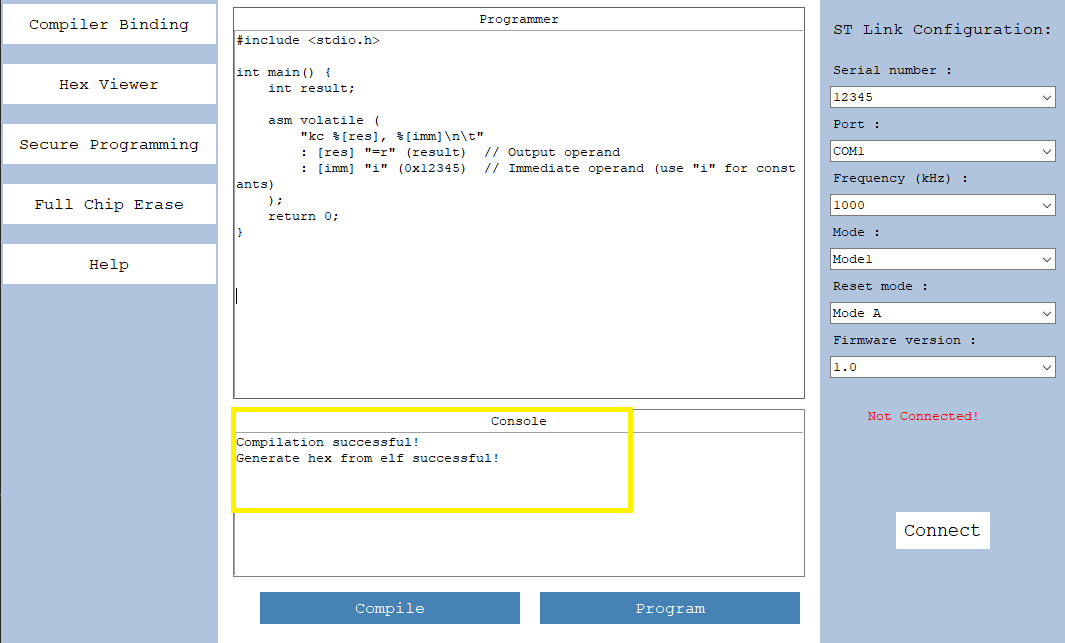
\includegraphics[width=\linewidth]{figures/fig_compile.png}
  \caption{Toolchain validation: compilation and ELF$\rightarrow$HEX generation with the custom instruction.}
  \label{fig:compile}
\end{figure}

\section{Firmware Inspection}
The host application provides a hex viewer to inspect generated images. Fig.~\ref{fig:hex}
illustrates the hex contents, supporting operator verification that the compiled image includes
the intended instruction sequence and metadata.

\begin{figure}[t]
  \centering
  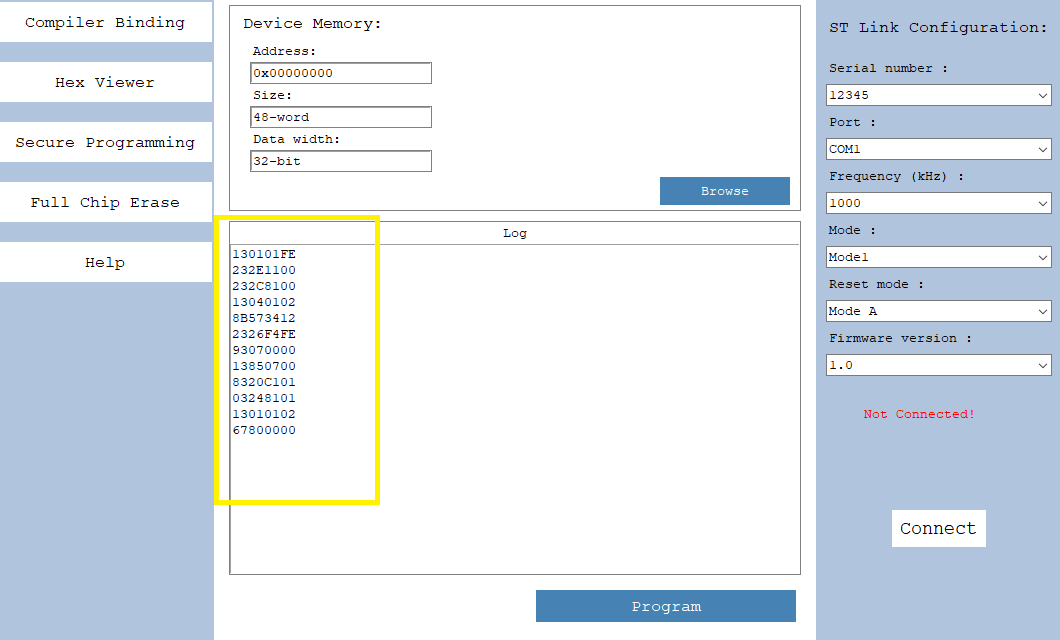
\includegraphics[width=\linewidth]{figures/fig_hex.png}
  \caption{HEX inspection: generated image viewed in the host application.}
  \label{fig:hex}
\end{figure}

\section{Authorization and Debug Enablement}
The core functional requirement is that debug access is released only after successful
authorization. Fig.~\ref{fig:auth} shows the key exchange with a successful match, followed by
debug enablement. This demonstrates that authorization is enforced on-device and not solely by
host-side policy.

\begin{figure}[t]
  \centering
  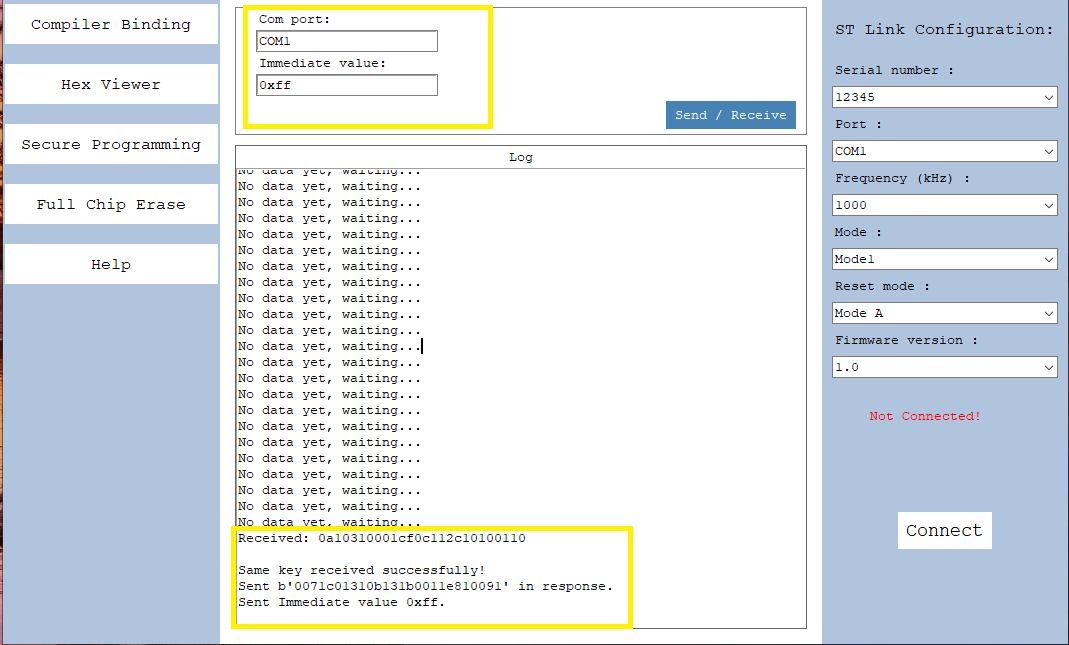
\includegraphics[width=\linewidth]{figures/fig_keymatch.png}\vspace{0.3ex}
  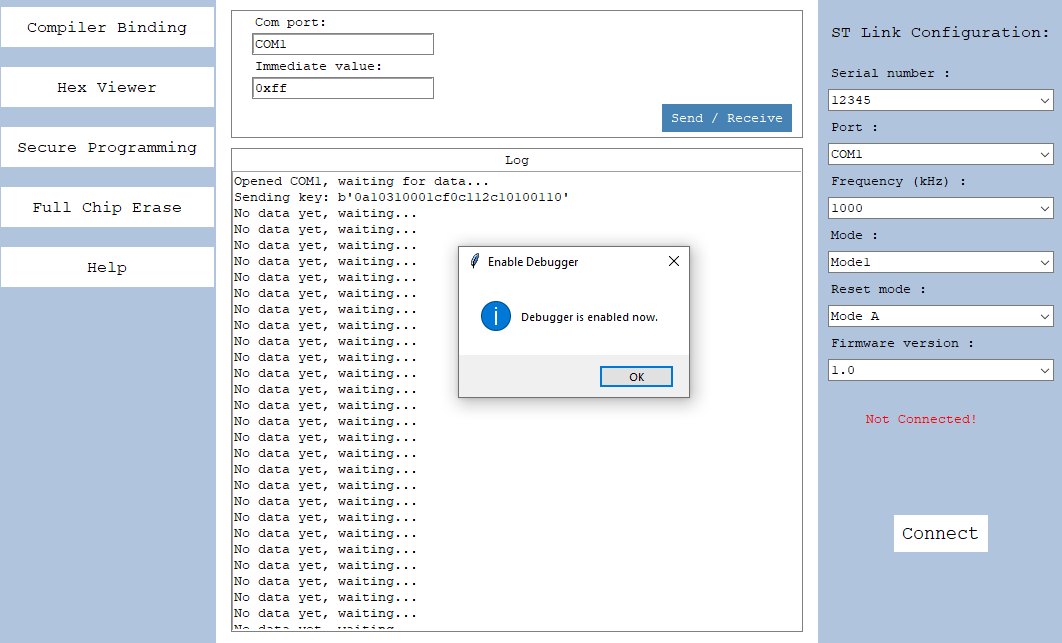
\includegraphics[width=\linewidth]{figures/fig_debugenabled.png}
  \caption{Authorization evidence: key match followed by debug enablement.}
  \label{fig:auth}
\end{figure}

\section{Fail-Stop Behavior on Mismatch}
To validate fail-stop behavior, an invalid key fragment is injected during the authorization
sequence. The device transitions to \textsf{HALT} and remains non-operational until reset,
preventing iterative probing within a single session. Fig.~\ref{fig:halted} shows a halted
device state after a mismatch.

\begin{figure}[t]
  \centering
  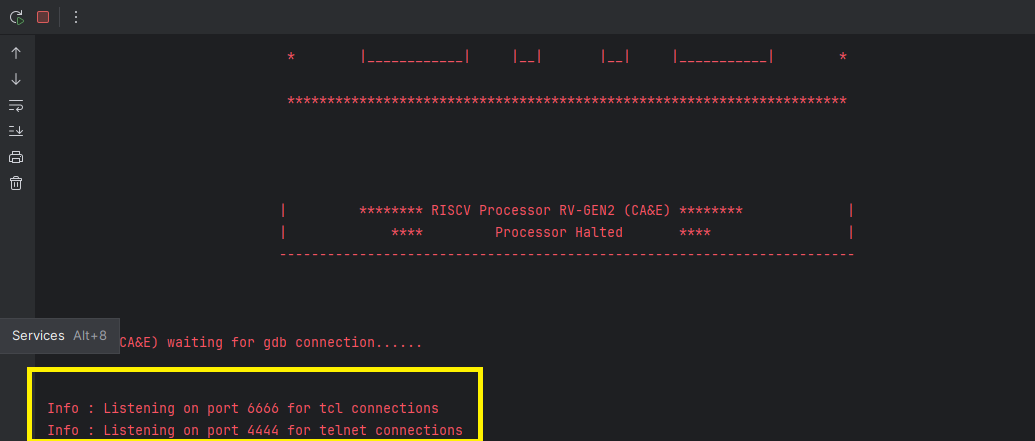
\includegraphics[width=\linewidth]{figures/fig_halted.png}
  \caption{Fail-stop evidence: device halted after authorization mismatch.}
  \label{fig:halted}
\end{figure}

\section{Programming Workflow Evidence}
The host workflow includes device connection, image load, and programming. Fig.~\ref{fig:program}
shows a successful connection state and a log entry indicating \texttt{load\_image} for the
compiled firmware, demonstrating that programming occurs under the expected authorization
conditions.

\begin{figure}[t]
  \centering
  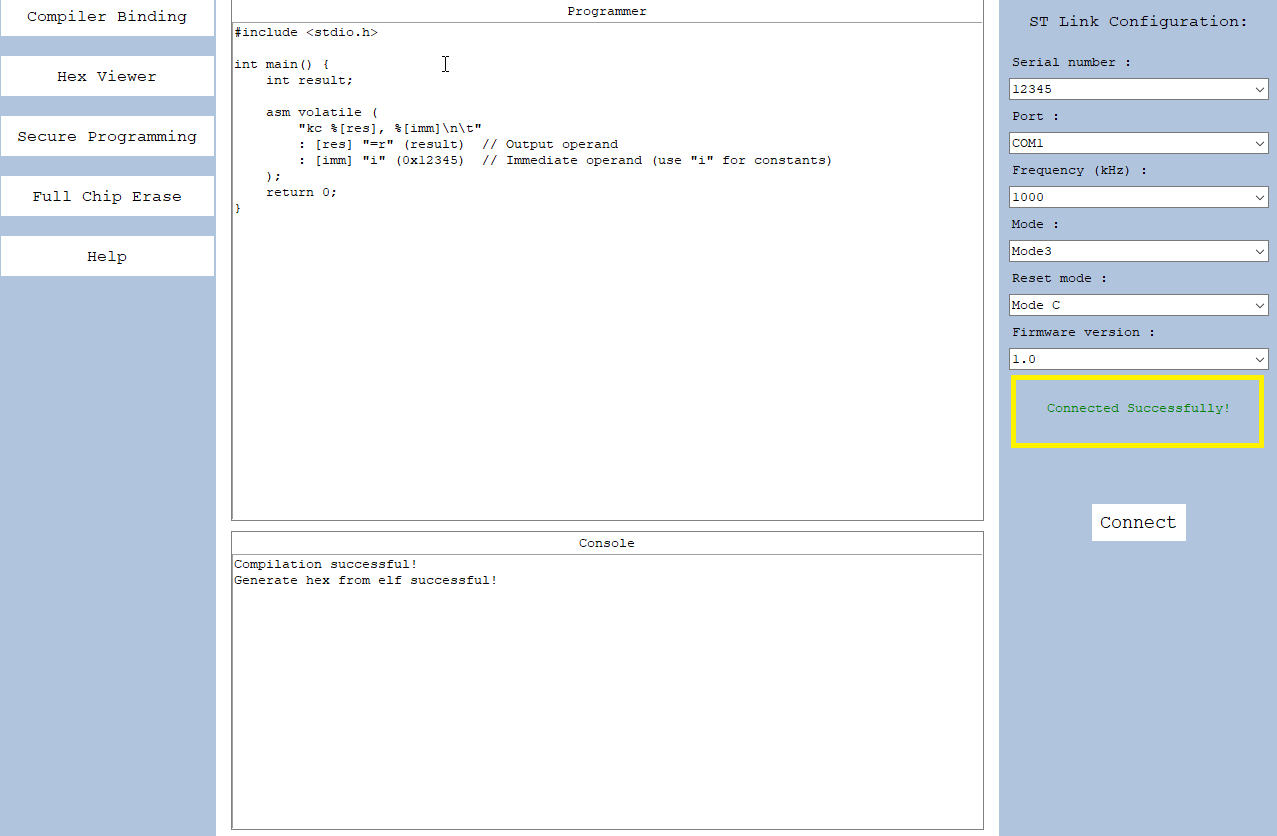
\includegraphics[width=\linewidth]{figures/fig_connected.png}\vspace{0.3ex}
  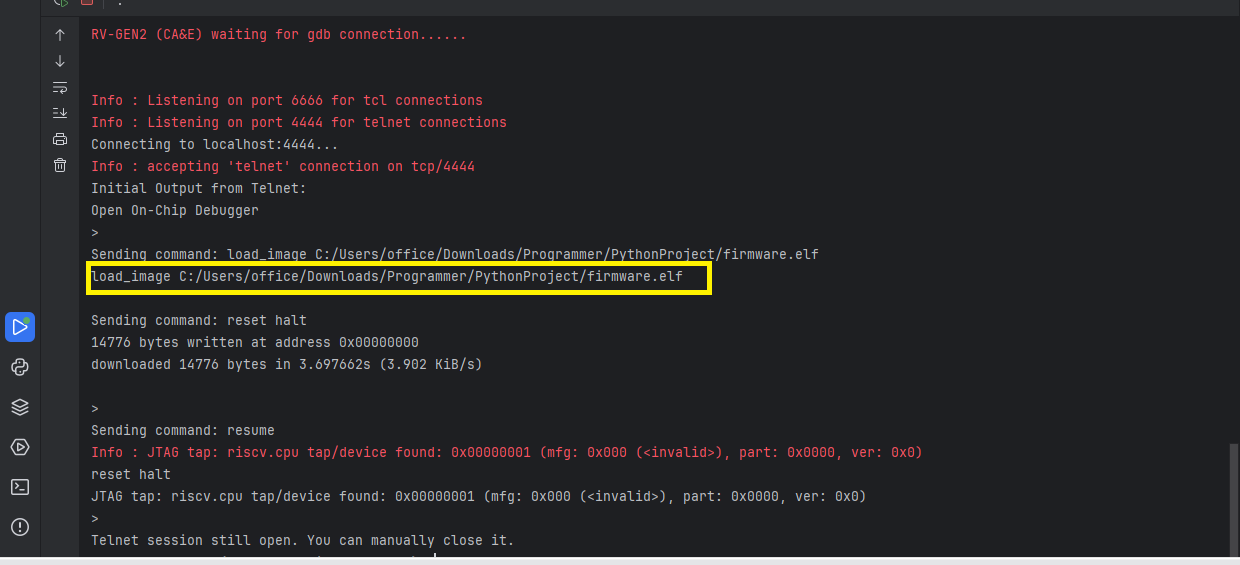
\includegraphics[width=\linewidth]{figures/fig_loadimage.png}
  \caption{Programming workflow evidence: successful connection and image load.}
  \label{fig:program}
\end{figure}

\section{Protocol Robustness Checks}
Additional checks validate that protocol deviations do not result in partial authorization.
Missing delimiters or out-of-order fragments reliably trigger a halt, and the host log records
the failure event. These checks demonstrate that authorization is not only dependent on a
correct key but also on adherence to the prescribed sequence, preventing malformed or replayed
traffic from enabling debug.

\section{Summary of Evidence}
Table~\ref{tab:thesis-results} summarizes the functional requirements and corresponding evidence.

\begin{table}[t]
  \centering
  \caption{Functional validation summary from collected artifacts.}
  \label{tab:thesis-results}
  \begin{tabular}{@{}ll@{}}
    \toprule
    \textbf{Requirement} & \textbf{Evidence} \\
    \midrule
    Custom instruction compiles and emits & Fig.~\ref{fig:compile} \\
    ELF$\rightarrow$HEX generation succeeds & Fig.~\ref{fig:compile} \\
    Hex inspection supported & Fig.~\ref{fig:hex} \\
    Key exchange and match visible & Fig.~\ref{fig:auth} \\
    Debug enabled only after match & Fig.~\ref{fig:auth} \\
    Device connection workflow supported & Fig.~\ref{fig:program} \\
    Programming log shows image load & Fig.~\ref{fig:program} \\
    \bottomrule
  \end{tabular}
\end{table}

\section{Reproducibility and Artifact Collection}
All evidence was collected from deterministic tool outputs and host logs. Build artifacts
include the compiler output, ELF$\rightarrow$HEX conversion logs, and disassembly listings that
show the \texttt{kc} opcode at the expected program point. Host-side logs capture key exchange
status, authorization decisions, and programming events. This collection enables repeatable
validation without requiring specialized measurement equipment.

\section{Limitations and Threats to Validity}
The evaluation emphasizes correctness of the enforcement path rather than quantitative
performance metrics. Timing overheads and power impact were not measured because the
authorization sequence is executed only during boot. The security claims rely on the
assumption that the protected NVM and comparator datapath are not subject to invasive
modification; violating these assumptions could bypass enforcement despite correct software
behavior.

\section{Discussion of Results}
The collected artifacts demonstrate that the authorization mechanism is enforced end-to-end:
the \texttt{kc} instruction is preserved in compiled images, authorization is required before
debug enablement, and programming events occur only after successful key verification. The
fail-stop behavior of the Authenticator FSM ensures that unsuccessful authorization attempts do
not release execution or debug capabilities. These results support the practicality of
instruction-triggered, key-gated control for embedded programming and debug access.
